% composition-renormalization.tex — TKF92 WFST composition, the
% relative-entropy (m-projection) fit, and the renormalization-group view.
% To be \input from tkf.tex.
%
% This is the MINIMAL appendix: just the setup needed to write the
% GGI->TKF92 matched-flow ODE on one page.  An earlier, much fuller
% version of this section (worked examples, the self-composition flow,
% the GGI-flow portrait, etc.) is preserved in
% composition-renormalization-detailed.tex for posterity.

\providecommand\evolu{u}
\providecommand\ggigen{G_{\mathrm{GGI}}}
\providecommand\ggikern{\mathbb{G}}
\providecommand\dkl[2]{D\!\left(#1\,\middle\|\,#2\right)}
\providecommand\ggi{\mathrm{GGI}}
\providecommand\nfragext{F}
\providecommand\nfragend{\bar F}
% Triad HMM macros (sec:comp-triad-hmm)
\providecommand\mat{\mathtt{M}}
\providecommand\ins{\mathtt{I}}
\providecommand\del{\mathtt{D}}
\providecommand\sta{\mathtt{S}}
\providecommand\fin{\mathtt{E}}
\providecommand\nul{\mathtt{N}}
\providecommand\ymx{a}
\providecommand\zmx{b}
\providecommand\ty[1]{a_{#1}}
\providecommand\tz[1]{b_{#1}}
\providecommand\triadstart{\mathtt{SS}}
\providecommand\stains{\mathtt{sI}}
\providecommand\matmat{\mathtt{MM}}
\providecommand\matins{\mathtt{mI}}
\providecommand\matdel{\mathtt{MD}}
\providecommand\insmat{\mathtt{IM}}
\providecommand\insins{\mathtt{iI}}
\providecommand\insdel{\mathtt{ID}}
\providecommand\delsta{\mathtt{Ds}}
\providecommand\delmat{\mathtt{Dm}}
\providecommand\delins{\mathtt{Di}}
\providecommand\deldel{\mathtt{Dd}}
\providecommand\triadend{\mathtt{EE}}
\providecommand\jointpairmatrix{\ymx}
\providecommand\condpairmatrix{\zmx}
\providecommand\jointpairhmm{\jointpairmatrix}
\providecommand\condpairhmm{\condpairmatrix}
\providecommand\fragext{\ext}
\providecommand\triadstates{\mathcal{S}_{\rm triad}}
\providecommand\texorpdfstring[2]{#1}
\providecommand\toLower{\mathrm{lc}}
\providecommand\ancestor{x}
\providecommand\descendant{y}
\providecommand\anc{\ancestor}
\providecommand\desc{\descendant}

\section{Composition, Relative-Entropy Fit, and the GGI--TKF92 Matched Flow}
\label{sec:composition-renorm}

This appendix gives the minimum setup required to write down the matched-flow
ODE for the best TKF92 surrogate of a GGI long-indel process as a function of
branch length $\evoltime$.  The objective is the conditional expected KL; the
flow is realised by an m-projection of the $13$-state \emph{Triad HMM}
$\jointpairhmm(\theta,\evoltime)\circ\condpairhmm(\theta_\ggi,d\evoltime)$.
Only the indel process is analysed (substitutions factor out and are
suppressed by working over a one-symbol alphabet).

\subsection{The Triad HMM and the \texorpdfstring{$U + V\,d\evoltime$}{U + V*dt} expansion}
\label{sec:comp-triad-hmm}

\paragraph{Compositional form.}
Let $\ymx=\jointpairmatrix(\insrate,\delrate,\fragext,\evoltime)$ be the
TKF92 joint Pair HMM transition matrix at surrogate parameters
$\theta=(\insrate,\delrate,\fragext)$ and branch length $\evoltime$; let
$\zmx=\condpairmatrix(\theta_\ggi,d\evoltime)$ be the GGI conditional
Pair HMM transition matrix for one infinitesimal step
$d\evoltime$ at GGI parameters $\theta_\ggi=(\insrate_0,\delrate_0,x,y)$
\begin{align*}
\tz{\sta\mat} = \tz{\mat\mat} &= 1 - (\insrate_0+\delrate_0)\,d\evoltime + o(d\evoltime), &
\tz{\sta\ins} = \tz{\mat\ins} &= \insrate_0\,d\evoltime, \\
\tz{\sta\del} = \tz{\mat\del} &= \delrate_0\,d\evoltime, &
\tz{\sta\fin} = \tz{\mat\fin} &= 1 - \insrate_0\,d\evoltime, \\
\tz{\ins\ins} &= x, & \tz{\ins\mat} = \tz{\ins\fin} &= 1-x, \\
\tz{\del\del} &= y, & \tz{\del\mat} &= 1-y, \\
\tz{\del\fin} &= 1, & \tz{\ins\del} = \tz{\del\ins} &= 0.
\end{align*}
The Triad is the composite transducer
$\jointpairhmm(\theta,\evoltime)\circ\condpairhmm(\theta_\ggi,d\evoltime)$
with the state space $\triadstates'=\triadstates \cup \{\insdel\}$ where
$\triadstates=\{\triadstart,\stains,\matmat,\matins,\matdel,\insmat,\insins,\delsta,\delmat,\delins,\deldel,\triadend\}$.
The cases in the state tuples $ik \in \triadstates'$ indicate which component(s) are updated on entry:
$\{\stains,\matins,\insins\}$ update the $\zmx$-component ($k$),
$\{\delsta,\delmat,\delins,\deldel\}$ update the $\ymx$-component ($i$), and
$\{\matmat,\matdel,\insmat,\insdel,\triadend\}$ update both components.

The resulting Triad transition matrix takes the form
$ Q'(\theta,\theta_\ggi,\evoltime,d\evoltime) \;=\; $

\noindent\resizebox{\textwidth}{!}{$
\left( \begin{array}{r|ccccccccccccc}
& \triadstart & \stains & \matmat & \matins & \matdel & \insmat & \insins & \insdel & \delsta & \delmat & \delins & \deldel & \triadend \\
\hline
\triadstart & 0 & \tz{\sta\ins} & \ty{\sta\mat}\tz{\sta\mat} & 0 & \ty{\sta\mat}\tz{\sta\del} & \ty{\sta\ins}\tz{\sta\mat} & 0 & \ty{\sta\ins}\tz{\sta\del} & \ty{\sta\del} & 0 & 0 & 0 & \ty{\sta\fin}\tz{\sta\fin}
\\ \stains & 0 & \tz{\ins\ins} & \ty{\sta\mat}\tz{\ins\mat} & 0 & \ty{\sta\mat}\tz{\ins\del} & \ty{\sta\ins}\tz{\ins\mat} & 0 & \ty{\sta\ins}\tz{\ins\del} & 0 & 0 & \ty{\sta\del} & 0 & \ty{\sta\fin}\tz{\ins\fin}
\\ \matmat & 0 & 0 & \ty{\mat\mat}\tz{\mat\mat} & \tz{\mat\ins} & \ty{\mat\mat}\tz{\mat\del} & \ty{\mat\ins}\tz{\mat\mat} & 0 & \ty{\mat\ins}\tz{\mat\del} & 0 & \ty{\mat\del} & 0 & 0 & \ty{\mat\fin}\tz{\mat\fin}
\\ \matins & 0 & 0 & \ty{\mat\mat}\tz{\ins\mat} & \tz{\ins\ins} & \ty{\mat\mat}\tz{\ins\del} & \ty{\mat\ins}\tz{\ins\mat} & 0 & \ty{\mat\ins}\tz{\ins\del} & 0 & 0 & \ty{\mat\del} & 0 & \ty{\mat\fin}\tz{\ins\fin}
\\ \matdel & 0 & 0 & \ty{\mat\mat}\tz{\del\mat} & \tz{\del\ins} & \ty{\mat\mat}\tz{\del\del} & \ty{\mat\ins}\tz{\del\mat} & 0 & \ty{\mat\ins}\tz{\del\del} & 0 & 0 & 0 & \ty{\mat\del} & \ty{\mat\fin}\tz{\del\fin}
\\ \insmat & 0 & 0 & \ty{\ins\mat}\tz{\mat\mat} & 0 & \ty{\ins\mat}\tz{\mat\del} & \ty{\ins\ins}\tz{\mat\mat} & \tz{\mat\ins} & \ty{\ins\ins}\tz{\mat\del} & 0 & \ty{\ins\del} & 0 & 0 & \ty{\ins\fin}\tz{\mat\fin}
\\ \insins & 0 & 0 & \ty{\ins\mat}\tz{\ins\mat} & 0 & \ty{\ins\mat}\tz{\ins\del} & \ty{\ins\ins}\tz{\ins\mat} & \tz{\ins\ins} & \ty{\ins\ins}\tz{\ins\del} & 0 & 0 & \ty{\ins\del} & 0 & \ty{\ins\fin}\tz{\ins\fin}
\\ \insdel & 0 & 0 & \ty{\ins\mat}\tz{\del\mat} & 0 & \ty{\ins\mat}\tz{\del\del} & \ty{\ins\ins}\tz{\del\mat} & \tz{\del\ins} & \ty{\ins\ins}\tz{\del\del} & 0 & 0 & 0 & \ty{\ins\del} & \ty{\ins\fin}\tz{\del\fin}
\\ \delsta & 0 & 0 & \ty{\del\mat}\tz{\sta\mat} & 0 & \ty{\del\mat}\tz{\sta\del} & \ty{\del\ins}\tz{\sta\mat} & 0 & \ty{\del\ins}\tz{\sta\del} & \ty{\del\del} & 0 & 0 & 0 & \ty{\del\fin}\tz{\sta\fin}
\\ \delmat & 0 & 0 & \ty{\del\mat}\tz{\mat\mat} & 0 & \ty{\del\mat}\tz{\mat\del} & \ty{\del\ins}\tz{\mat\mat} & 0 & \ty{\del\ins}\tz{\mat\del} & 0 & \ty{\del\del} & 0 & 0 & \ty{\del\fin}\tz{\mat\fin}
\\ \delins & 0 & 0 & \ty{\del\mat}\tz{\ins\mat} & 0 & \ty{\del\mat}\tz{\ins\del} & \ty{\del\ins}\tz{\ins\mat} & 0 & \ty{\del\ins}\tz{\ins\del} & 0 & 0 & \ty{\del\del} & 0 & \ty{\del\fin}\tz{\ins\fin}
\\ \deldel & 0 & 0 & \ty{\del\mat}\tz{\del\mat} & 0 & \ty{\del\mat}\tz{\del\del} & \ty{\del\ins}\tz{\del\mat} & 0 & \ty{\del\ins}\tz{\del\del} & 0 & 0 & 0 & \ty{\del\del} & \ty{\del\fin}\tz{\del\fin}
\\ \triadend & 0 & 0 & 0 & 0 & 0 & 0 & 0 & 0 & 0 & 0 & 0 & 0 & 0
\end{array} \right)
$}

Eliminating the $\insdel$ state gives the $12\times 12$ transition matrix for the null-eliminated triad,
$Q_{ij} = Q'_{ij} + Q'_{i\ \insdel} Q'_{\insdel j} / (1 - Q'_{\insdel\ \insdel})$.

The null-eliminated transition matrix is linear in $d\evoltime$:
\begin{equation}
\label{eq:triad-AB}
Q(\theta,\theta_\ggi,\evoltime,d\evoltime) \;=\;
U(\theta,\evoltime) \;+\; V(\theta,\theta_\ggi,\evoltime)\,d\evoltime
\;+\; O(d\evoltime^2),
\end{equation}
with $U$ collecting the entries of $Q$ that are $d\evoltime$-independent
and $V$ collecting the $d\evoltime$ coefficients.  Defining
$C:=(I-U)^{-1}$, to first order
\begin{equation}
\label{eq:triad-resolvent}
(I-Q)^{-1} \;=\; C \;+\; (CVC)\,d\evoltime \;+\; O(d\evoltime^2).
\end{equation}

\paragraph{Coarse-graining.}
The coarse-graining $C_{\rm proj}:\triadstates\to\{\sta,\mat,\ins,\del,\fin\}$
projects Triad states $(\triadstart,\matmat,\triadend)$ to $(\sta,\mat,\fin)$;
$\{\stains,\matins,\insmat,\insins\}$ to $\ins$;
and $\{\delsta,\delmat,\delins,\deldel\}$ to $\del$.
With Triad state $\insdel$ marginalized, the map yields coarse-grained counts $m_{XY}$.
In matrix form, with
$\Sigma^{XY}_{ab}=1$ iff $C_{\rm proj}(a)=X,C_{\rm proj}(b)=Y$,
\begin{equation}
\label{eq:triad-counts}
m_{XY}(\theta,\theta_\ggi,\evoltime,d\evoltime) \;=\;
\sum_{a,b}\bigl[(I-Q)^{-1}\bigr]_{\triadstart\,a}\;Q_{ab}\;\Sigma^{XY}_{ab}\;
\bigl[(I-Q)^{-1}\bigr]_{b\,\triadend}.
\end{equation}

\subsection{Objective: conditional expected KL}
\label{sec:comp-cond-kl}

We minimise the conditional expected KL between descendant distributions,
with the expectation taken over the surrogate's ancestor marginal:
\begin{equation}
\label{eq:cond-kl-objective}
\overline{D}(\theta,\evoltime) \;=\;
\mathbb{E}_{P_T(s;\theta)}\!\Bigl[\dkl{P_\ggi(s'\!\mid\! s;\evoltime)}
{P_T(s'\!\mid\! s;\theta,\evoltime)}\Bigr].
\end{equation}

The matched flow is the self-composition m-projection
\begin{equation}
\label{eq:matched-flow}
\theta(\evoltime+d\evoltime) \;=\; \arg\min_{\theta'}\;
\overline{D}\bigl(\,\jointpairhmm(\theta(\evoltime),\evoltime)\circ\condpairhmm(\theta_\ggi,d\evoltime)\;\big\|\;\jointpairhmm(\theta',\evoltime+d\evoltime)\,\bigr).
\end{equation}

\subsection{Three equivalent ODE systems}
\label{sec:comp-ode}

\paragraph{The $\Delta$ operator.}
For any function $f(\theta,\theta_\ggi,\evoltime,d\evoltime)$ that is regular
at $d\evoltime\!=\!0$, write its $d\evoltime$ expansion
$f = f^{(0)} + \Delta[f]\,d\evoltime + O(d\evoltime^2)$, so
\begin{equation}
\label{eq:delta-def}
\Delta[f] \;:=\; \frac{\partial f}{\partial(d\evoltime)}\bigg|_{d\evoltime=0}.
\end{equation}
Applied along the matched flow $\evoltime\mapsto\theta(\evoltime)$, this is
the total $\evoltime$-derivative of $f$: the m-projection
condition~\eqref{eq:matched-flow} forces
$df/d\evoltime = \Delta[f](\theta(\evoltime),\evoltime)$, since the source
at $(\evoltime,d\evoltime)$ becomes the surrogate at $\evoltime+d\evoltime$.

\paragraph{Transition counts.}
Expand~\eqref{eq:triad-counts} via~\eqref{eq:triad-resolvent}.  The surrogate's
own counts at $(\theta,\evoltime)$ and the leading $d\evoltime$ perturbation are
\begin{equation}
\label{eq:ode-counts-explicit}
m^{(0)}_{XY}(\theta,\evoltime) \;=\;
\sum_{a,b}C_{\triadstart,a}\,U_{ab}\,\Sigma^{XY}_{ab}\,C_{b,\triadend},
\end{equation}
\begin{equation}
\label{eq:delta-m}
\Delta m_{XY}(\theta,\theta_\ggi,\evoltime) \;=\;
\sum_{a,b}\Sigma^{XY}_{ab}\Bigl[(CVC)_{\triadstart,a}\,U_{ab}\,C_{b,\triadend}
\,+\, C_{\triadstart,a}\,V_{ab}\,C_{b,\triadend}
\,+\, C_{\triadstart,a}\,U_{ab}\,(CVC)_{b,\triadend}\Bigr].
\end{equation}
The count flow ODE is then
\begin{equation}
\label{eq:ode-counts}
\frac{d m_{XY}}{d\evoltime} \;=\; \Delta m_{XY}(\theta(\evoltime),\evoltime),
\qquad m_{XY}(0)=0,
\end{equation}
with $\theta(\evoltime)$ recovered at each step from $m(\evoltime)$ via the
TKF92 M-step (see below).  At every $\evoltime$, the flowing counts
$m_{XY}(\evoltime)$ coincide with the surrogate's self-consistent value
$m^{(0)}_{XY}(\theta(\evoltime),\evoltime)$ from~\eqref{eq:ode-counts-explicit}.

\paragraph{BDI sufficient statistics.}
Let $X\in\{B,D,S,\nfragext,\nfragend\}$ index the five TKF92 BDI
sufficient statistics (insertions $B$, deletions $D$, time-integrated
fragment count $S$, fragment extensions $\nfragext$, fragment terminations
$\nfragend$).  Each is a linear functional of the coarse-grained counts
$m_{XY}$ under the standard TKF92 BDI map, so $\Delta[X]$ is the same map
applied to $\Delta m_{XY}$.  The flow is
\begin{equation}
\label{eq:ode-suffstats}
\frac{dE_T[X]}{d\evoltime} \;=\; \Delta[X](\theta(\evoltime),\evoltime),
\qquad E_T[X](0)=0,
\qquad X\in\{B,D,S,\nfragext,\nfragend\}.
\end{equation}

\paragraph{TKF92 parameters.}
Differentiating the TKF92 M-step formulas
$\insrate=E[B]/(E[S]+T)$, $\delrate=E[D]/E[S]$, and
$\fragext=E[\nfragext]/(E[\nfragext]+E[\nfragend])$ along the flow gives the
equivalent system in the natural parameters:
\begin{equation}
\label{eq:ode-params}
\boxed{\;
\begin{aligned}
\dot{\insrate} &= \frac{\Delta[B] - \insrate\,(\Delta[S]+1)}{E_T[S]+\evoltime} \\[1pt]
\dot{\delrate} &= \frac{\Delta[D] - \delrate\,\Delta[S]}{E_T[S]} \\[1pt]
\dot{\fragext} &= \frac{(1-\fragext)\,\Delta[\nfragext] - \fragext\,\Delta[\nfragend]}{E_T[\nfragext]+E_T[\nfragend]}
\end{aligned}\;}
\end{equation}
where the $+1$ in the $\insrate$ numerator is the immortal-link clock
($dT/d\evoltime=1$), and $T=\evoltime$ is the total observation time.

The three systems~\eqref{eq:ode-counts}, \eqref{eq:ode-suffstats}, and
\eqref{eq:ode-params} are equivalent (related by the linear BDI map and the
TKF92 M-step).  Form~\eqref{eq:ode-suffstats} is the numerically convenient
one; \eqref{eq:ode-params} relates most directly to the TKF92 surrogate one
actually uses; and \eqref{eq:ode-counts} makes the algebraic structure
(rational in $C$, linear in $V$) most visible.

\subsection{Boundary conditions at \texorpdfstring{$\evoltime\to0^+$}{t -> 0+}}
\label{sec:comp-boundary}

At $\evoltime=0$ the surrogate's conditional descendant distribution is the
identity, so the conditional KL~\eqref{eq:cond-kl-objective} vanishes for any
$\theta$; the boundary value $\theta(0^+)$ is therefore pinned by the
leading-$O(\evoltime)$ KL rate.  In the per-residue (large-$L$) limit the
insertion KL alone is minimised by $\fragext=y$ and the deletion KL alone by
$\fragext=x$.  The joint per-residue minimum is the weighted average
\begin{equation}
\label{eq:boundary-r}
\fragext^\ast(0) \;=\; \frac{\insrate_0\,y(1-x) + \delrate_0\,x(1-y)}
{\insrate_0\,(1-x) + \delrate_0\,(1-y)},
\end{equation}
with the corresponding rate boundaries
\begin{equation}
\label{eq:boundary-rates}
\insrate^\ast(0) \;=\; \frac{\insrate_0}{1-\fragext^\ast(0)},
\qquad
\delrate^\ast(0) \;=\; \frac{\delrate_0}{1-\fragext^\ast(0)}.
\end{equation}
Eq.~\eqref{eq:boundary-r}--\eqref{eq:boundary-rates} are the principled
$\evoltime\to0^+$ initial conditions for~\eqref{eq:ode-params}; the
$E_T[X]$ in~\eqref{eq:ode-suffstats} start at zero and the parameters are
recovered by the L'H\^opital limits
$\insrate(0^+)=\Delta[B](\theta(0),0)/(\Delta[S](\theta(0),0)+1)$, and
similarly for $\delrate(0^+),\fragext(0^+)$, evaluated at $\theta(0)$
from~\eqref{eq:boundary-r}--\eqref{eq:boundary-rates}.

\paragraph{Validity of $\fragext^\ast(0) \in (0,1)$.}  Eq.~\eqref{eq:boundary-r}
is the per-residue minimiser of the leading KL term, but for arbitrary
$(\insrate_0,\delrate_0,x,y)$ it need not lie in $(0,1)$.  Writing
$1-\fragext^\ast(0) = (D-N)/D$ with $D=\insrate_0(1-y)+\delrate_0(1-x)$ and
$N=\insrate_0\,y(1-x)+\delrate_0\,x(1-y)$, a short calculation gives
\begin{equation}
\label{eq:rstar-validity}
1-\fragext^\ast(0)
\;=\; \frac{\insrate_0(1-2y+xy) + \delrate_0(1-2x+xy)}{D}.
\end{equation}
Either bracket is negative when the corresponding length parameter exceeds
$1/(2-\text{other})$ (e.g.\ $1-2x+xy<0$ iff $x>1/(2-y)$), and the
combined numerator can become negative when one bracket dominates.  In
particular, the GGI reversibility condition $\insrate_0\,y(1-y)=\delrate_0\,x(1-x)$
permits asymmetric solutions with $x>1/2$, $y<1/2$ (or vice versa), and
for sufficiently extreme combinations even $\insrate_0\le\delrate_0$ does
not save the bound: the leading-order picture predicts $\fragext^\ast(0)>1$,
i.e.\ no physical TKF92 boundary value exists.  The closed-form
trajectory~\eqref{eq:r-closedform} below then has $k<0$ and $\fragext(\evoltime)$
diverges; the closed form must be regarded as extrapolating outside its
region of validity.  Practical fitters should either restrict to GGI
shapes with $\fragext^\ast(0)\in(0,1)$ or refuse to score in the
out-of-region tail (we observed this when fitting Pfam: a $\rho\!\le\!1$
constraint on $\insrate_0/\delrate_0$ alone does not suffice).

\subsection{Empirically, all three drift modestly; \texorpdfstring{$\fragext$}{r} moves most}
\label{sec:comp-tameness}

Numerical integration of~\eqref{eq:ode-params} at Pfam-fitted TKF92 scale
$(\insrate,\delrate,\fragext)\!\approx\!(0.046,\,0.047,\,0.68)$,
inferring the underlying GGI rates from the boundary as
$(\insrate_0,\delrate_0)=\bigl((1-\fragext)\insrate,(1-\fragext)\delrate\bigr)\!\approx\!(0.0145,\,0.0148)$,
and sweeping $(x,y)$ over the one-parameter family of Pfam-consistent
GGI shapes (those for which~\eqref{eq:boundary-r} yields
$\fragext^\ast\!=\!0.683$), gives the envelope across $\evoltime\in[0.05,10]$:
\begin{equation}
\label{eq:pfam-ranges}
\insrate(\evoltime)\!\in\![0.0410,\,0.0450],\quad
\delrate(\evoltime)\!\in\![0.0416,\,0.0460],\quad
\fragext(\evoltime)\!\in\![0.580,\,0.679],
\end{equation}
with relative spreads of $9.4\%$, $10.1\%$, and $15.7\%$ respectively.  All
three drift, $\fragext$ most.  Two practical consequences:
\begin{itemize}[nosep]
\item Freezing $(\insrate,\delrate)$ at the boundary values during the
$\fragext$-flow incurs at most a $\sim\!10\%$ rate-parameter error over
$\evoltime\in[0.05,10]$, and reduces the three-parameter
system~\eqref{eq:ode-params} to a single $\fragext$-ODE.  This is a
useful approximation when $\evoltime$ is varied (e.g.\ over a phylogeny
with branch lengths in the Pfam range) but a fixed TKF92 fit is desired
for the rate parameters.
\item The branch-length dependence that genuinely cannot be ignored is
$\fragext(\evoltime)$: a single CherryML fit at a representative
$\evoltime$ misses up to $\sim\!17\%$ of $\fragext$'s actual variation.
\end{itemize}
\paragraph{First-order fragment-counting closed form for $\fragext(\evoltime)$.}
A first-order argument tracks how a single GGI event changes the surrogate's
expected extension and termination counts $F, \nfragend$ in the alignment-count
view.  A GGI insertion of length $\ell\sim\mathrm{Geom}(y)$ at a random link
adds an $\ins$-block, contributing on average $E[(1{-}\fragext)\Delta F -
\fragext\Delta\nfragend] = (1-\fragext)/(1-y) - (1+\fragext)$ per event.  A GGI
deletion of length $\ell\sim\mathrm{Geom}(x)$ at a random residue contributes
$(1-\fragext)/(1-x) - (1+\fragext)$ by the analogous accounting (with the
self-loop $\ins{\to}\ins$ contributions of insertion blocks playing the role of
the $\del{\to}\del$ contributions of deletion blocks).  Combining with the
per-link and per-residue event rates gives the leading slope
\begin{equation}
\label{eq:rdot-firstorder}
\dot\fragext \;=\; (1{-}\fragext)\!\left[\tfrac{\insrate_0}{1-y}+\tfrac{\delrate_0}{1-x}\right]
\;-\; (1{+}\fragext)(\insrate_0+\delrate_0).
\end{equation}
Evaluated at the boundary $\fragext=\fragext^\ast(0)$, the bracket collapses by
the boundary identity (using
$(1-\fragext^\ast)= (1-x)(1-y)(\insrate_0+\delrate_0)/[\insrate_0(1-x)+\delrate_0(1-y)]$
to show that
$(1-\fragext^\ast)[\insrate_0/(1-y)+\delrate_0/(1-x)] = \insrate_0+\delrate_0$),
giving the strikingly simple initial slope
\begin{equation}
\label{eq:rdot-clean}
\dot\fragext(0^+) \;=\; -\fragext^\ast(0)\,(\insrate_0+\delrate_0),
\qquad\text{i.e.}\qquad
\left.\tfrac{d\log\fragext}{d\evoltime}\right|_{0^+} \;=\; -(\insrate_0+\delrate_0).
\end{equation}
Equation~\eqref{eq:rdot-firstorder} is a separable linear ODE
$\dot\fragext = (A-B) - (A+B)\fragext$ with $A = \insrate_0/(1-y)+\delrate_0/(1-x)$
and $B = \insrate_0+\delrate_0$, integrating to the closed form
\begin{equation}
\label{eq:r-closedform}
\boxed{\;\fragext(\evoltime) \;\approx\; \fragext_\infty
\;+\; \bigl(\fragext^\ast(0)-\fragext_\infty\bigr)\,
\exp\!\Bigl[-(\insrate_0+\delrate_0)\,\tfrac{2-\fragext^\ast(0)}{1-\fragext^\ast(0)}\,\evoltime\Bigr],\quad
\fragext_\infty = \tfrac{\fragext^\ast(0)}{2-\fragext^\ast(0)}\;}
\end{equation}
where the fixed point $\fragext_\infty$ and decay rate
$k=(\insrate_0+\delrate_0)(2-\fragext^\ast)/(1-\fragext^\ast)$ both follow from
the same boundary identity.

\paragraph{Reparameterisation in terms of $(\insrate(0),\delrate(0),\fragext(0))$.}
In practice the user often has a TKF92 fit at a representative branch length
(e.g.\ CherryML) but no GGI shape parameters $(x, y)$.  The boundary relations
$\insrate_0=(1-\fragext(0))\insrate(0)$ and $\delrate_0=(1-\fragext(0))\delrate(0)$
let us recast~\eqref{eq:r-closedform} entirely in terms of the TKF92
boundary values:
\begin{equation}
\label{eq:r-closedform-tkf}
\boxed{\;
\fragext(\evoltime) \;\approx\; \fragext_\infty
\;+\; \bigl(\fragext(0)-\fragext_\infty\bigr)\,e^{-k\evoltime},\quad
\fragext_\infty = \tfrac{\fragext(0)}{2-\fragext(0)},\quad
k = (\insrate(0)+\delrate(0))(2-\fragext(0)).\;}
\end{equation}
The leading slope is
$\left.d\fragext/d\evoltime\right|_{0^+} = -\fragext(0)(1-\fragext(0))(\insrate(0)+\delrate(0))$.
Note that the rate parameters $\insrate_0,\delrate_0$ of the underlying GGI
do not appear separately --- only the TKF92 sum $\insrate(0)+\delrate(0)$
--- and the GGI shape $(x,y)$ does not appear at all.  The slaved rate
trajectories follow directly:
$\insrate(\evoltime) \approx \insrate(0)(1-\fragext(0))/(1-\fragext(\evoltime))$,
$\delrate(\evoltime) \approx \delrate(0)(1-\fragext(0))/(1-\fragext(\evoltime))$.
This is the most directly usable form when a TKF92 fit is available.

For Pfam-scale parameters
($\fragext(0)\!=\!0.683$, $\insrate(0)+\delrate(0)\!=\!0.0926$):
$\fragext_\infty\!=\!0.52$, $k\!=\!0.12$.  Comparison with the full
three-parameter flow~\eqref{eq:ode-params}: $\fragext$ values agree to
$<\!2\%$ for $\evoltime\lesssim 1$, to $\sim\!10\%$ at $\evoltime\!=\!10$
(Figure~\ref{fig:pfam-closedform}).  At branch lengths $\evoltime\gtrsim 50$
the full flow develops a non-monotonic kink (a local minimum of $\fragext$
followed by a slow rise) that is a higher-order effect not captured by
this leading-order linearisation; for typical phylogenies the kink is well
outside the relevant branch-length range.

\paragraph{Fragment coherence half-life.}
The rate constant $k$ in~\eqref{eq:r-closedform-tkf} sets a natural
time-scale for fragment coherence under TKF92:
\begin{equation}
\label{eq:t-half}
\boxed{\;t_{1/2}^{\mathrm{frag}} \;\equiv\; \frac{\ln 2}{k}
  \;=\; \frac{\ln 2}{(\insrate(0)+\delrate(0))\,(2-\fragext(0))}
  \;=\; \frac{\ln 2\,(1-\fragext^\ast(0))}
              {(\insrate_0+\delrate_0)(2-\fragext^\ast(0))}\;}
\end{equation}
(The TKF92-parametrisation form, useful when a TKF92 boundary fit
$(\insrate(0),\delrate(0),\fragext(0))$ is available, and the
GGI-parametrisation form, useful when starting from the underlying
$(\insrate_0,\delrate_0,x,y)$, are equivalent under the boundary slaving
$\insrate(0)=\insrate_0/(1-\fragext^\ast(0))$,
$\delrate(0)=\delrate_0/(1-\fragext^\ast(0))$,
$\fragext(0)=\fragext^\ast(0)$.)
This is the branch length over which $\fragext(\evoltime)-\fragext_\infty$
decays to half its initial value.  For $\evoltime \ll t_{1/2}^{\mathrm{frag}}$
the constant-$\fragext$ (vanilla TKF92) approximation is excellent;
for $\evoltime \gtrsim t_{1/2}^{\mathrm{frag}}$ the
GGI-induced $\fragext$ flow is the dominant correction.
The single-component Pfam aligned fit
($\insrate\approx 0.030$, $\delrate\approx 0.030$, $\fragext\approx 0.65$)
gives $k\approx 0.081$, $t_{1/2}^{\mathrm{frag}}\approx 8.6$, well above
typical Pfam cherry times (median $\evoltime\approx 0.76$); a median
cherry traverses only $\sim 6\%$ of $\fragext(0)-\fragext_\infty$,
making the indivisible-fragment assumption near-exact across the Pfam
corpus.  A $K\!=\!20$ Pfam-mixture fit's components span
$t_{1/2}^{\mathrm{frag}}\in[3.4, 15.0]$
(weighted mean $\approx 9.5$); even the fastest-flow component
moves only $\sim 14\%$ of the available flow over a median cherry.
This is the proximate reason that constant-$\fragext$ TKF92 fits to
Pfam are competitive with GGI-steered TKF92 fits: at Pfam composition,
the data simply lacks the temporal span needed to resolve the GGI
$\fragext$-flow signal.  Datasets with larger $\evoltime/t_{1/2}^{\mathrm{frag}}$,
either through faster ($\insrate$, $\delrate$) or longer branches, would
break the degeneracy.

For applications outside the phylogenetic regime the three-parameter
ODE~\eqref{eq:ode-params} is integrated numerically, either by a
finite-difference $m$-projection or by analytically including the
immortal-link clock ($\partial_T E[X]$) and parameter-drift
($\nabla_\theta E[X]\cdot\dot\theta$) contributions to $\dot E_T[X]$.

\begin{figure}[t]
\centering
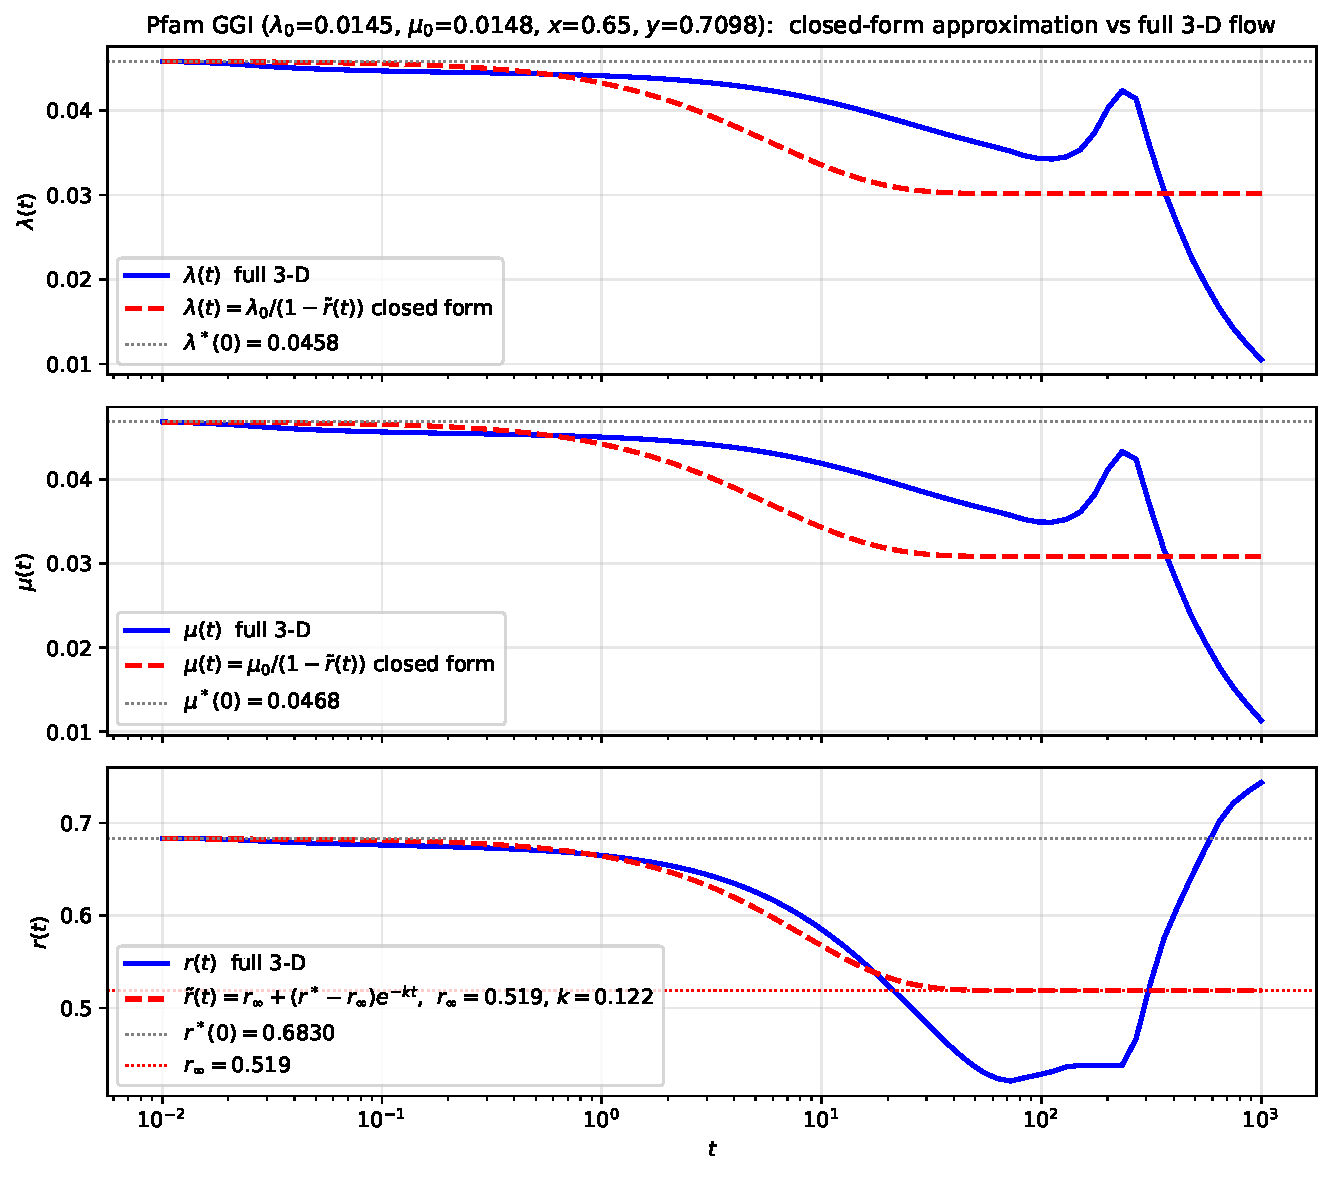
\includegraphics[width=0.85\textwidth]{pfam_closedform}
\caption{Pfam-scale ($\insrate_0\!\approx\!0.0145$, $\delrate_0\!\approx\!0.0148$,
$x\!=\!0.65$, $y\!=\!0.71$) flow out to $\evoltime=10^3$.  Full three-parameter
flow~\eqref{eq:ode-params} (solid blue) vs the leading-order closed
form~\eqref{eq:r-closedform} with the slaved rates
$\insrate(\evoltime)=\insrate_0/(1-\fragext(\evoltime))$,
$\delrate(\evoltime)=\delrate_0/(1-\fragext(\evoltime))$ (dashed red).
Agreement is tight up to $\evoltime\!\sim\!5$.  The closed form asymptotes to
$\fragext_\infty=\fragext^\ast(0)/(2-\fragext^\ast(0))\!=\!0.52$; the full flow
dips below this near $\evoltime\!\sim\!70$ and then rises back, a higher-order
kink the linearised closed form does not capture.
For typical phylogenies the relevant branch-length range
($\evoltime\!\lesssim\!10$) lies well inside the regime where the closed
form is accurate.}
\label{fig:pfam-closedform}
\end{figure}

\paragraph{Single-parameter (fragment-length) flow versus triple-parameter
(rates and fragment-length) flow.}
\label{para:single-param-flow}
The matched-flow ODE \eqref{eq:ode-params} can be integrated for all
three of $(\insrate, \delrate, \fragext)$ jointly --- the
\emph{triple-parameter flow} --- or under the truncation that holds
$\insrate, \delrate$ fixed at their boundary values
$\insrate_T(0) = \insrate_0/(1-\fragext^\ast(0))$,
$\delrate_T(0) = \delrate_0/(1-\fragext^\ast(0))$ and integrates only
$\fragext$:
\begin{equation}
\label{eq:frozen-rate-r}
\dot\fragext(\evoltime) \;=\; \frac{(1-\fragext)\,\Delta[\nfragext] -
\fragext\,\Delta[\nfragend]}{E_T[\nfragext]+E_T[\nfragend]}
\bigg|_{\,\insrate=\insrate_T(0),\,\delrate=\delrate_T(0)}.
\end{equation}
We refer to this truncation as the \emph{single-parameter
(fragment-length) flow}.  The two ODEs agree to leading order in
$\evoltime$, and~\eqref{eq:r-closedform-tkf} is the leading-order
closed-form solution of either.  Beyond leading order the two flows
diverge.  The triple-parameter flow integrates a coupled three-dimensional
system in which the $(\insrate, \delrate)$ drift back-couples into the
$\dot\fragext$ formula, and the resulting $\fragext$ trajectory can
become non-monotonic at moderate $\evoltime$; the single-parameter flow
remains monotonic by construction and stays well-fit by
\eqref{eq:r-closedform-tkf} throughout.  At the matched-flow projection
geometry the two flows define different cumulative projection-error
rates, but their conditional KL to the underlying GGI process is
comparable across phylogenetic branch lengths.  We adopt the
single-parameter flow as the recommended approximation: it is
algebraically clean, captures the matched-flow geometry of $\fragext$,
and admits the closed-form solution boxed below.

\paragraph{Closed-form TKF92 approximation to GGI: summary.}
\label{para:tkf92-closed-form-box}
Collecting the recommended approximation for the matched-flow surrogate
of a GGI process with rates $\insrate_0,\delrate_0$ and extension
parameters $x$ (deletion) and $y$ (insertion):
\medskip
\noindent\fbox{\parbox{0.97\textwidth}{%
\textbf{Closed-form TKF92 surrogate for GGI.}\\[2pt]
Given GGI parameters $(\insrate_0,\delrate_0,x,y)$, the recommended
constant-rate TKF92 surrogate has
\begin{align*}
\fragext^\ast(0) &= \frac{\insrate_0\,y\,(1-x) + \delrate_0\,x\,(1-y)}
                         {\insrate_0\,(1-x) + \delrate_0\,(1-y)}, \\[2pt]
\insrate_T &\equiv \frac{\insrate_0}{1-\fragext^\ast(0)},
\qquad
\delrate_T \equiv \frac{\delrate_0}{1-\fragext^\ast(0)}, \\[2pt]
\fragext(\evoltime) &= \fragext_\infty + (\fragext^\ast(0)-\fragext_\infty)\,
   e^{-k\,\evoltime}, \\[2pt]
\fragext_\infty &= \frac{\fragext^\ast(0)}{2-\fragext^\ast(0)},
\qquad
k = (\insrate_0+\delrate_0)\,\frac{2-\fragext^\ast(0)}{1-\fragext^\ast(0)}.
\end{align*}
The rates $\insrate_T,\delrate_T$ are held constant; only $\fragext$
evolves with $\evoltime$.  The Pair HMM transition matrix is then
$\tkftrans'(\insrate_T,\delrate_T,\fragext(\evoltime),\evoltime)$.
The branch-length scale on which $\fragext(\evoltime)$ is changing is
the fragment coherence half-life
$t_{1/2}^{\mathrm{frag}}=\ln 2/k$~\eqref{eq:t-half}.
}}
\medskip

\paragraph{Numerical comparison on Pfam parameters.}
Figure~\ref{fig:pfam-flow-1param} compares the single-parameter
flow~\eqref{eq:frozen-rate-r} and the closed-form
approximation~\eqref{eq:r-closedform-tkf} against per-$\tau$ ML fits of
TKF92 (via the conditional WFST) to Gillespie simulations on the Pfam
joint-native fit ($\insrate_0\!=\!0.01061$, $\delrate_0\!=\!0.01065$,
$x\!=\!0.641$, $y\!=\!0.638$).  The top panel shows $\fragext(\evoltime)$
under the single-parameter flow, the closed-form approximation, and
the per-$\tau$ ML fit; the fragment coherence half-life
$t_{1/2}^{\mathrm{frag}}$~\eqref{eq:t-half} is marked.  The bottom panel shows the per-$\tau$
conditional KL
$D(P_\ggi(\desc\mid\anc)\,\|\,P_{\tkftrans''_T}(\desc\mid\anc))$ in
bits per cherry on a linear $y$ axis; the ancestor singlet is factored
out analytically as
$D_\mathrm{cond} = D(P_\ggi(\anc,\desc)\,\|\,P_\tau(\anc,\desc)) -
D(P_\ggi(\anc)\,\|\,P_\tau(\anc))$, so the comparison reflects only the
surrogate's error on the descendant-given-ancestor distribution.  The
per-$\tau$ Gillespie cherry budget is adapted to the small-$\evoltime$
event-paucity regime: at branch length $\evoltime$ the expected number
of indel decisions per cherry is approximately $R\evoltime$ where
$R \approx (L_\anc+1)\insrate_0/(1-y) + L_\anc\delrate_0/(1-x)$ is the
per-cherry equilibrium decision rate, so for a target absolute SE of
$\sigma$ on the per-$\tau$ ML estimate of $\fragext$ we set
$N_\text{cherries}(\evoltime) = \max(N_\text{floor},
\fragext(1-\fragext)/(\sigma^{2}R\evoltime))$.  At $\sigma=0.005$,
$N_\text{floor}=3000$, this peaks at $\sim 3.8\cdot 10^{5}$ cherries
near $\evoltime=0.005$ and floors at $3000$ once $R\evoltime$ saturates.
Error bars are over $5$ independent simulations.  The two surrogates
give comparable conditional KL throughout the phylogenetic range, with
both growing monotonically as the constant-rate TKF92 approximation
becomes increasingly imperfect at long branch lengths; the
single-parameter flow tracks the per-$\tau$ ML fit on $\fragext$ to
within sampling error.

\begin{figure}[t]
\centering
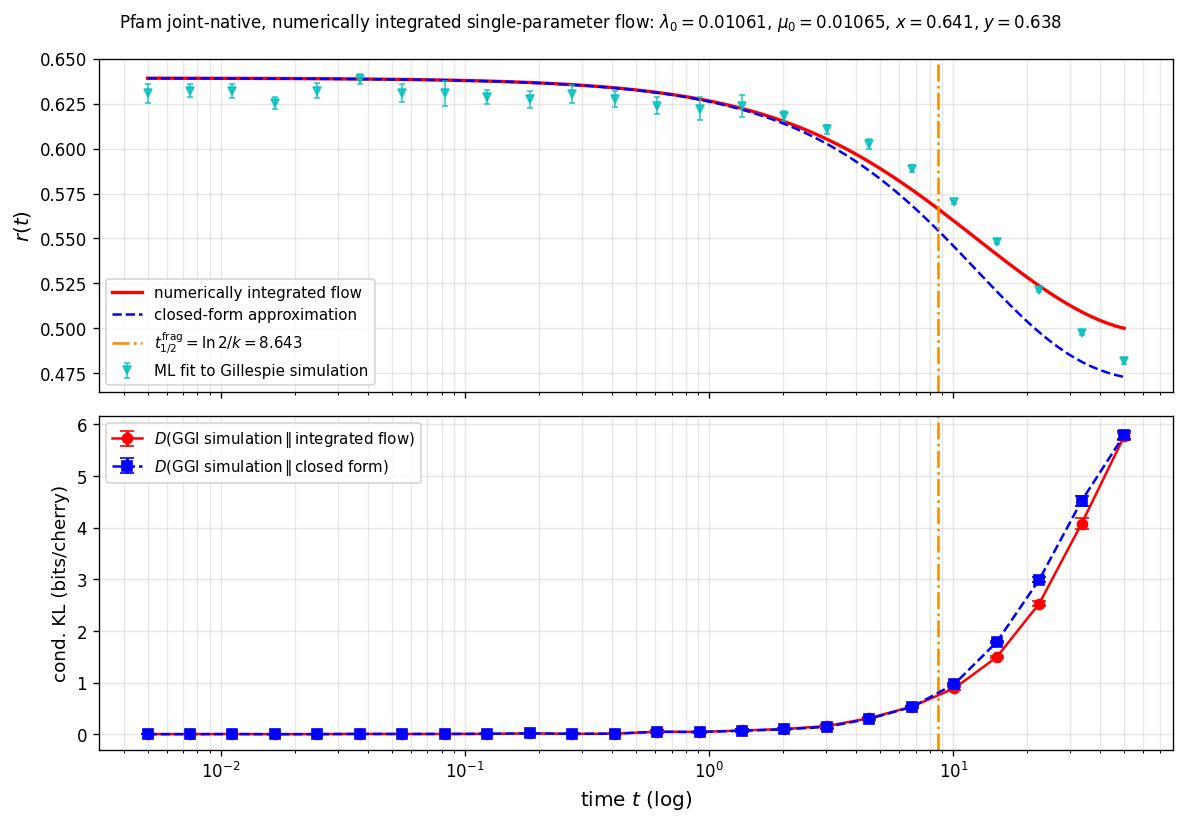
\includegraphics[width=0.95\textwidth]{pfam_flow_1param}
\caption{Pfam joint-native ($\insrate_0\!=\!0.01061$,
$\delrate_0\!=\!0.01065$, $x\!=\!0.641$, $y\!=\!0.638$),
$\evoltime\!\in\![0.005,\,50]$.  Top panel: $\fragext(\evoltime)$
trajectories under (i)~the numerically-integrated single-parameter
(fragment-length) flow~\eqref{eq:frozen-rate-r} (red solid),
(ii)~the closed-form approximation~\eqref{eq:r-closedform-tkf} (blue
dashed), and (iii)~per-$\tau$ ML fit of TKF92 to the Gillespie data via
the conditional WFST (cyan $\blacktriangledown$).  The dark-orange
dash-dotted vertical line marks the fragment coherence half-life
$t_{1/2}^{\mathrm{frag}}$~\eqref{eq:t-half}.  Bottom panel: per-$\tau$ conditional KL
$D(P_\ggi(\desc\mid\anc)\,\|\,P_{\tkftrans''_T}(\desc\mid\anc))$ per
cherry, in bits, on linear $y$ axis; the ancestor distribution is
factored out analytically.  The per-$\tau$ Gillespie cherry budget is
adapted ($\sigma=0.005$, $N_\text{floor}=3000$; see surrounding text);
error bars are over $5$ independent simulations.}
\label{fig:pfam-flow-1param}
\end{figure}
